\documentclass{turabian-researchpaper}

\usepackage[utf8]{inputenc}
\usepackage{csquotes, ellipsis}
\usepackage{graphicx}
\usepackage{wrapfig}

\usepackage[pass, letterpaper]{geometry}

\usepackage{biblatex-chicago}
\usepackage{biblatex}
\addbibresource{works-cited.bib}

\title{Deviance Through Divinity}
\subtitle{An Analysis of Saint Hildegard's Illustrations and Her Peculiar Rise to Power}
\author{Ryan Heffelman}
\course{ARH 3760}
\date{October 26, 2023}

\begin{document}
\maketitle

\section{Introduction}

    What does it take to be a successful historical female artist? In the case of Saint Hildegard von Bingen, divine intervention. In a truly one of a kind manner, Saint Hildegard literally transcended the gender constraints imposed upon her by a patriarchal society, and she managed to do it in the most unlikely time and place imaginable: amongst devout religious people of a male-oriented Latin church in the 12th century. Saint Hildegard was not just a significant female artist, but a significant \emph{person}, and one who should not be overlooked. In this paper I'd like to talk about the intricacies and properties of Saint Hildegard's unique position as a visionary and how it relates to gender history, as well as providing analysis on her illustrations with a particular focus on \emph{The Universe}, attempting to tackle its widespread misportrayal.


\section{Background Information on Saint Hildegard}

    There are many fields you can attribute Saint Hildegard as being a part of, but the truth is she predates our modern conceptions of all of them. In her intellectual pursuits she was not setting out to be an astronomer, a scientist, a philosopher, a linguist, etc. She sought knowledge for the purest of motives: to know. Her goal was not to know about any one particular field, or to know more than anyone else, but to answer the mysteries of the universe and become closer to God. Hildegard was born in the year 1098 and three years later, she experienced the first in a series of visions that would continue throughout the course of her life.\autocite[77]{motc} At age 42 she experienced a vision of God instructing ``write down that which you see and hear'', so she created her first major work: Scivias.\autocite{scivias}\autocite[8]{vw} Scivias is an illuminated manuscript containing illustrations of her visions alongside descriptions of and commentary on them, and perhaps her most well known work. She went on to produce several more volumes on visionary theology, many musical compositions, plays, and two pioneering books on scientific natural history: \emph{Physica} and \emph{Causae et Curae}. She died in 1179 at age 81 which is an extraordinarily long life for being in medieval Europe, nearly triple the life expectancy at that time (double if you eliminate those who died before adulthood).\autocite[25]{bitel} All in all she lived an incredibly interesting and rich life with many accomplishments, particularly relative to other women and people in her time period.

\section{A Problem With the Interpretation of Saint Hildegard as an Artist}

    In order to explain this problem I'd like to introduce a quote from Saint Hildegard's Scivias Book I following a paragraph claiming God detests incest: ``I am explaining this by this person [Hildegard], to whom this human operation is unknown; she is receiving this explanation not from human knowledge, but from God''.\autocite{scivias}\autocite[82]{scivias} This is to say that her works are created by God through her as a proxy. God is expressing himself through her as a medium. If that's the case, then wouldn't that make her no more of an artist than Picasso's paintbrush is? Can \emph{she} really be seen as the artist of her works if it is God acting through her? Is this what allows her to remain in operation in a time and place so intolerant of female artists? One must tolerate her actions because her actions are divine actions, to speak against her would be blasphemy. As far as I can see there are two ways around this problem, the first of which being the Atheist way: the Catholic God is not real therefore God cannot be acting through her and her actions are no ones but her own. The second way being the idea that while her illustrations are based on visions she experienced from God, she still went through the creative process of artistically representing what she's perceived, therefore she is an artist in the same way any impressionist painter is.
    

\section{Hildegard von Bingen: Just a Girl}

    When put in their historical context, Hildegard's actions deviate egregiously from the prevailing norm. In medieval Europe, women occupied a strictly subordinate role to men regardless of class, with women quite literally being considered property of their nearest male relative under law.\autocite{khan} In addition, it was a commonly held belief that women were intellectually inferior to men, stemming from the biblical idea that woman was created for the sake of man. While certainly taboo, nuns in particular practicing painting and illustration was not entirely uncommon. What was uncommon however, was Hildegard's role as a preacher and instructor: ``a woman must be a learner, listening quietly and with due submission. I do not permit a woman to be a teacher, nor must a woman domineer over a man; she should be quiet''.\autocite[52]{chadwick} Saint Hildegard was anything but quiet, having gone on several extensive public ``preaching tours'', she did an extraordinarily good job at making her voice heard (Figure 4). Furthermore she faced relatively little resistance from The Church and society, considering the deviation from conventional norms. What's interesting is that she reinforced these same exact norms in her teaching and rhetoric. Hildegard existed within and played upon a gap in logic originating from the flawed beliefs of her society. The contemporary belief was that women were intellectually unremarkable, therefore Hildegard, a woman, cannot be intellectually remarkable, which serves to prove her status as a visionary. I suspect Hildegard was aware of this gap and intentionally exploited it. She played cunningly into the female inferiority dogma, frequently referring to herself as an ``unlearned woman'', incapable of formulating such elaborate philosophies and profound biblical interpretations. I could not help but draw parallels between her actions and the modern day ``I'm just a girl'' trend. She went around preaching that women should keep quiet and not voice their opinions, and when questioned on the inherent contradiction of that existence, resorted to a response essentially equivalent to ``but I'm just a girl''. In analyzing her visions through a modern lens, we know that at least some of her theological works were influenced to an extent by other scholars and their works such as Aristotle and his \emph{Meteorologica}.\autocite[66]{singer} In addition, her works on scientific natural history amongst other things do not claim to be of divine origin but rather Hildegard's own intellect and reasoning, proving that she is in fact intelligent in her own right, regardless of how you feel about her visionary claim.
    \linebreak[4]
    It should be noted, however, the ethical complications that arise due to her unique position; perhaps she's not the feminist icon that she appears to be on the surface. Reinforcing the doctrine of a misogynistic and overbearingly patriarchal society was a condition for her power in said society, but do the ends justify the means? By putting herself in power through preaching female submission, chastity, and inferiority and providing proof of its virtue through supposed direct communication with God, she took away power from all other women. I personally believe that she came out ahead because ultimately she served to prove the opposite-- that women have the capability to be equal or greater than men if given the opportunity.


\section{\emph{The Universe} and Saint Hildegard's Astronomical legacy}

    In medieval times, astronomy was chaotic and unsolved, it assumed a position of marked prominence. Saint Hildegard was a notable figure in many fields of medieval study, one of which being astronomy. In fact she's essentially the only documented female astronomer from the vast time period of the middle ages (but it's likely there were many undocumented). An illustration of a theoretical model of the universe by a woman in this time period is one of a kind (Figure 1). When looking at any of her illustrations it is important to keep in mind that they are designed to be interpreted through pictorial analogy and mythology as opposed to literal representation of described phenomena, the reasoning in her theological works is almost exclusively a priori. A nice example of this would be how in Figure 3, the surface of the earth in the south west was thought to be uninhabitable because it is in the mouth of a dragon (Figure 3).\autocite{singer} Another would be the ``torches'' or discolored looking stars aligned along the central axis of The Universe depicting the moon, Venus, Mercury, the sun, Mars, Jupiter, and Saturn (Figure 1). The commentary following The Universe illustration in Scivias states that ``The visible and temporal is a manifestation of the invisible and eternal''. This idea resonates with the distinction between the Kantian phenomenal and the noumenal-- the phenomenal domain implies the existence of but says nothing about the noumenal domain.\autocite[94]{scivias} The illustration represents a \emph{universal} union of the domains with both being shown; the terrestrial orb or microcosm in the center and the rest being her depiction of the macrocosm or as she puts it the ``invisible and eternal''.


\section{Cosmic Egg?}

    Many people have claimed that \emph{The Universe} intentionally resembles the female reproductive system, and it corroborates a common Christian depiction of gender archetypes: the universe is feminine and masculinity is the master of the universe (Figure 1).\autocite{scivias} I'd like to argue that no, this was not Hildegard's intention, at least not her conscious intention. First of all, in her many pages of commentary on the symbolism of the illustration including sections on the overall shape, she does not once acknowledge the resemblance to the female reproductive system. In fact she refers to it repeatedly as a ``vast instrument, round and shadowy, in the shape of an egg''.\autocite[94]{scivias} She states that the shape of the egg symbolizes the progression of humanity through God, how at first humanity was rough and simple in it's actions, and was later ``enlarged'' in its morals through the Old and New Testament. Second, many so-called \emph{mappae mundi}, or medieval European maps of the world, depict earth as an oval. It's likely that she came to her conception of the egg shaped world through a misunderstanding of these maps.\autocite[65]{singer} This is further proven by the fact that the orientation of her map matches that of other mappae mundi from the time period, East and West on the top and bottom, North and South on the left and right. Finally, the illustration in question is not her only attempt at depicting the universe, just her first one. Her later more mature and refined works such as \emph{Liber Divinorum Operum} feature illustrations of a symmetrical sphere shaped universe (Figure 2).\autocite{ISHVBS} The incongruity in the configuration of her theoretical universes suggests a potential inaccuracy in one of the models. It's safe to assume that Hildegard favored the spherical model, given its plural and later occurrence in her life.
    \linebreak[4]
    One cannot help but draw the parallel to Georgia O'Keeffe and the seemingly strange compulsion to attribute sexual intentions unto female artists, even in cases where those sexual intentions are not there, and there's not much evidence to suggest that they would be. People love a good controversy, and how scandalous would it be if indeed Hildegard von Bingen, a Saint, was secretly painting vaginas for the Catholic church under the guise of divine visions from God? In my research I read through an article making the argument that not only does The Universe depict a woman's genitalia, but that Hildegard had a secret lesbian relationship with her young assistant, Richardis von Stade.\autocite{nihil}

\section{Conclusion}
    
    Saint Hildegard von Bingen's life is a fascinating story of a clever abbess maneuvering the complex interplay of gender dynamics within medieval European society, going from a subjected position to even a privileged one. She did this by leveraging her position as a visionary appealing to the values of society at the time. Beyond this she had an incredibly active and independent mind, she was certainly a notable figure in an array of different fields of study, and she ought to be accredited for her contributions even in the domains which she pursued due to divine command. Her illustrations, which were created under the context of theological visions contain profound symbolism, but not quite the kind symbolism that's so often attributed to her. I argue the perhaps controversial view that The Universe illustration is not in fact vulvar for a variety of reasons, one of which being that it was never acknowledged in the contemporary moment. In my research of Saint Hildegard's legacy it was evident that her visionary prowess, intellectual independence, and artistic contributions defy the constraints of her time, pushing us to appreciate the enduring impact of her unique position and perspective in history.

\begin{figure}
    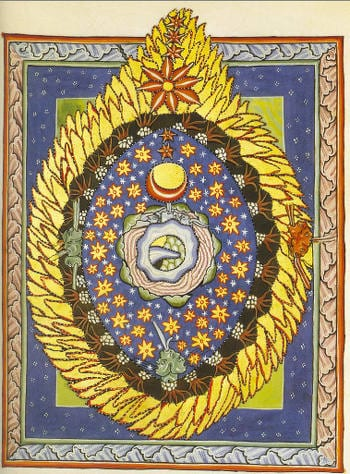
\includegraphics{universe.jpeg}
    \caption{The Universe\autocite{hh}}
    \label{The Universe}
\end{figure}

\begin{figure}
    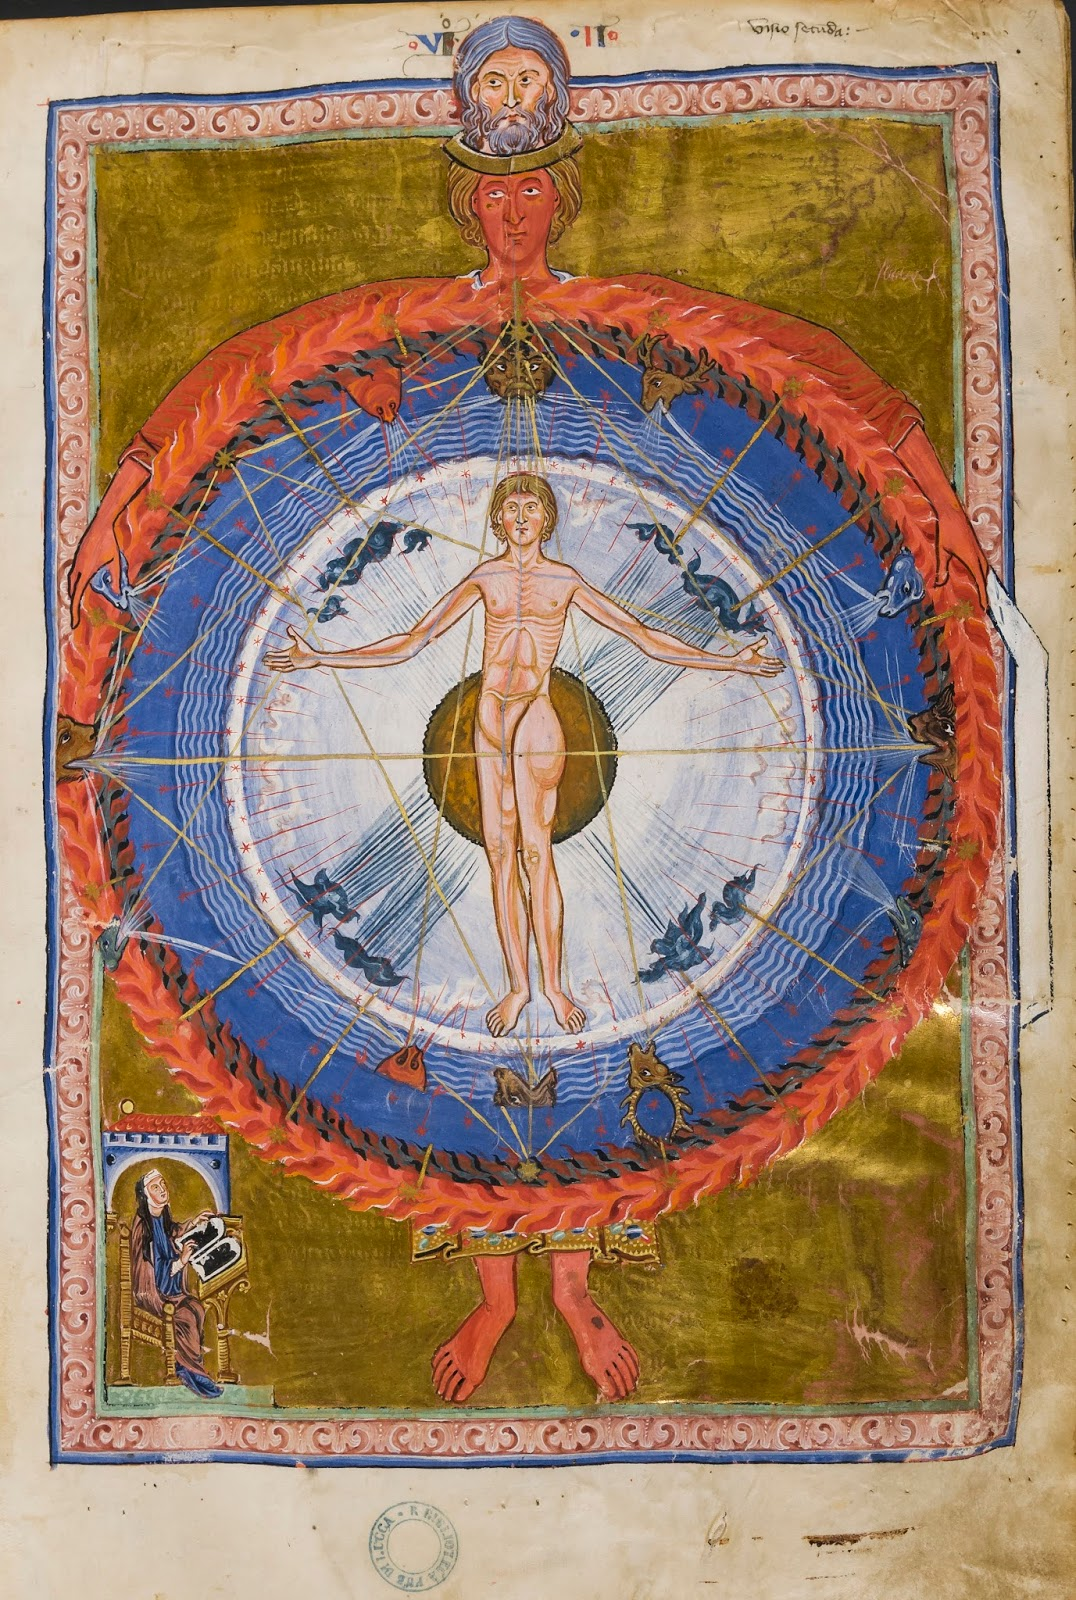
\includegraphics[scale=0.4]{liber.jpg}
    \caption{The Cosmic Spheres and Human Being\autocite{ISHVBS}}
    \label{The Cosmic Spheres}
\end{figure}

\begin{figure}
    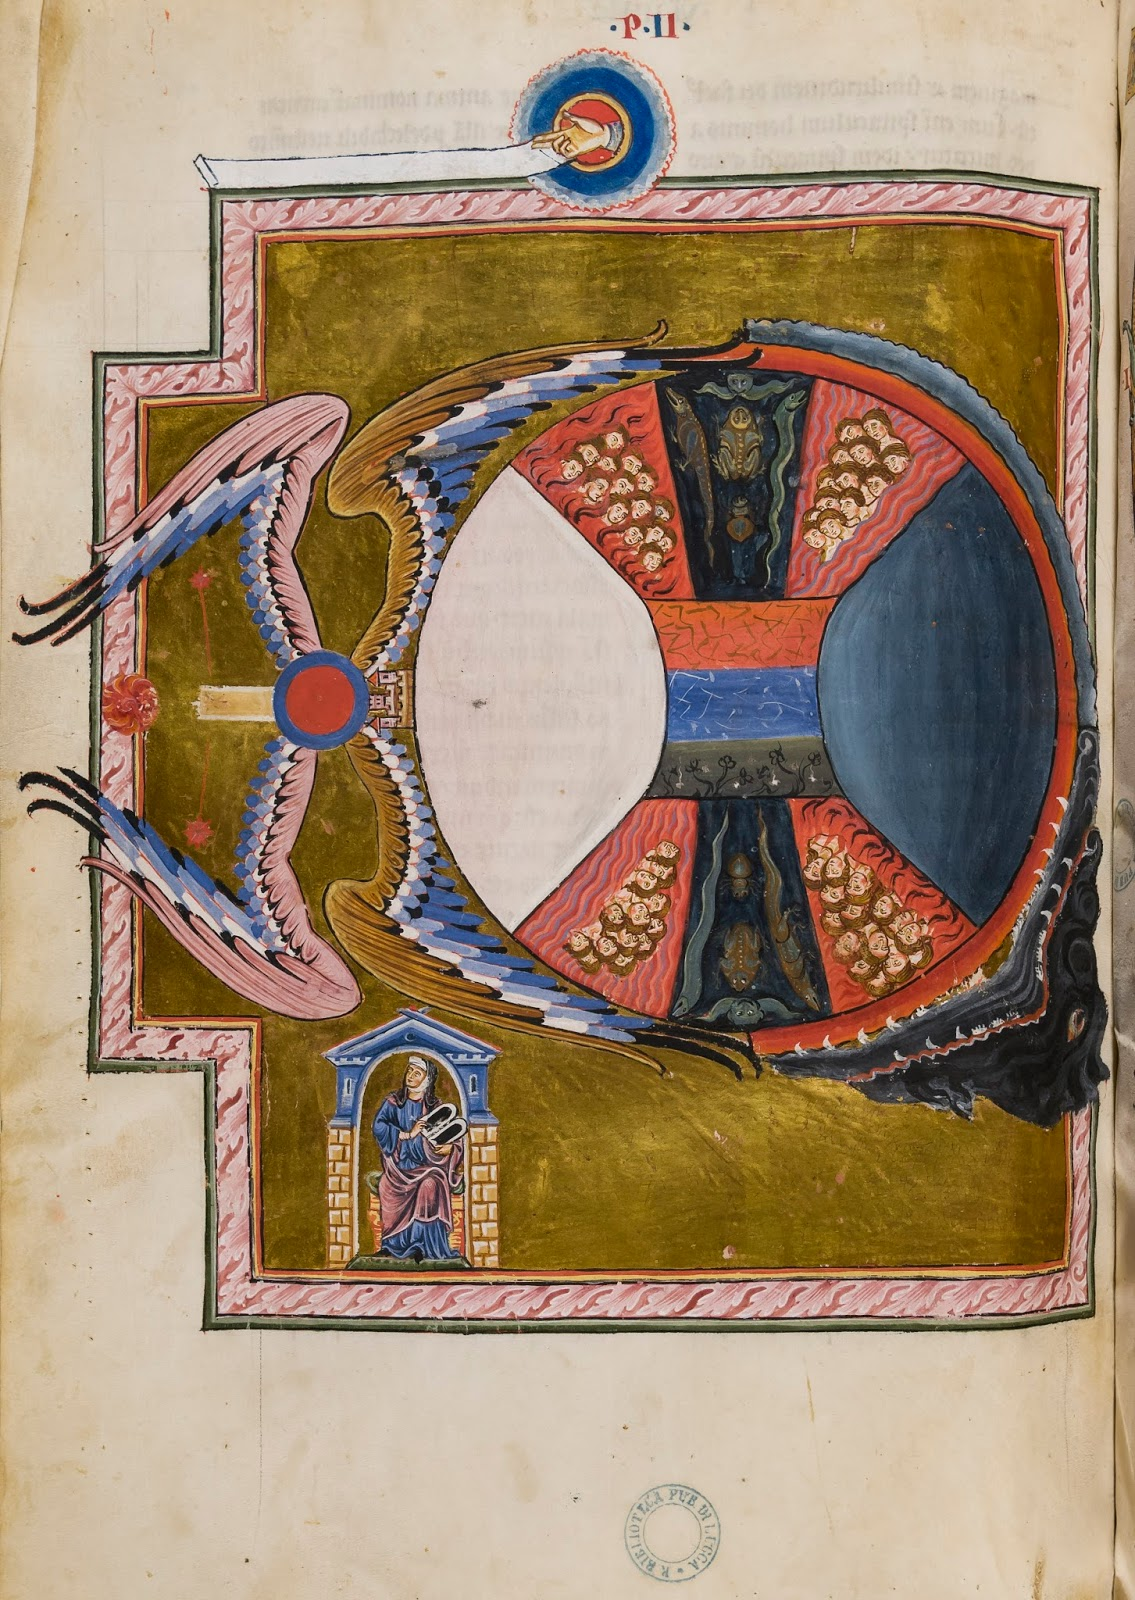
\includegraphics[scale=0.4]{dragon.jpg}
    \caption{\emph{The Parts of the Earth: Living, Dying, and Purgatory.}\autocite{ISHVBS}}
    \label{The Parts of the Earth}
\end{figure}

\begin{figure}
    
\includegraphics{Hildegard_map.jpg}
    \caption{\emph{Hildegard's Germany}\autocite{ISHVBS}}
    \label{Hildegard's Germany.}
\end{figure}

\clearpage
\printbibliography
\end{document}